\documentclass[12pt]{article}
\usepackage{setspace,fix-cm,times,indentfirst,custom,graphicx,report}
\usepackage[margin=1in]{geometry}

\renewcommand*\contentsname{\textsf{Table of Contents}}
\renewcommand*\listtablename{\textsf{List of Tables}}
\renewcommand*\listfigurename{\textsf{List of Figures}}
\renewcommand*\refname{\textsf{References}}

\begin{document}

\begin{titlepage}
\begin{center}
\textsc{\LARGE University of Waterloo}\\[1.5cm]
\textsc{\Large Software Engineering 101 Final Project}\\[0.5cm]

\HRule \\[0.4cm]
{\huge \bfseries Recon Scribbler}\\
\HRule \\[1.5cm]

\begin{minipage}{0.4\textwidth}
\begin{flushleft} \large
\emph{Authors:}\\
Kevin \textsc{Carruthers}\\
Yi Fei \textsc{Chen}\\
In Soo \textsc{Choo}\\
YoungJin \textsc{Kim}\\
Shida \textsc{Li}\\
Da \textsc{Wei}
\end{flushleft}
\end{minipage}
\begin{minipage}{0.4\textwidth}
\begin{flushright} \large
\emph{User IDs:} \\
kcarruth, \textsc{20463098}\\
yf8chen, \textsc{20485683}\\
ischoo, \textsc{20460165}\\
yj42kim, \textsc{20474159}\\
s22li, \textsc{20456719}\\
d4wei, \textsc{20477847}
\end{flushright}
\end{minipage}

\vfill
{\large November 23, 2012}
\end{center}
\end{titlepage}

\section*{\fontsize{16}{16}\textsf{Letter of Submittal}}
\onehalfspacing
\thispagestyle{empty}


\newpage

\pagenumbering{roman}
\tableofcontents\newpage
\listoffigures
\addcontentsline{toc}{section}{List of Figures}
\newpage
\listoftables
\addcontentsline{toc}{section}{List of Tables}
\newpage
\pagenumbering{arabic}

\section*{\fontsize{16}{16}\textsf{1 Executive Summary}}
\addcontentsline{toc}{section}{Executive Summary}
\onehalfspacing

In this project, we programmed and modelled the scribbler, a multifunction robot, to take on the role of an un-manned recon robot. This type of robot is particularly useful for exploring an unapproachable environment exposed to hazardous material or extreme conditions such as intense heat or freezing temperatures. Through the integration of our creativity, programming skills, and engineering principles, we organized the scribblers and the myro librarys diverse functions such as its IR sensors, movement ability, camera, and picture processing\cite{parallax} to create a comprehensive system that allows the scribbler to explore an area unguided, and return relevant information of the area structure to the user in the form of real-time map updates on the computer screen.\\

One of our group members prior knowledge and experiences in 2D mapping from a game called Minecraft helped us transfer the data obtained by the robot to a 2D map: in effect, mapping the data collected by the robot on a surface onto a 2D map.\\

The robot successfully explored an open area, using an obstacle-avoiding algorithm. The algorithm consisted of a simple path-finding code along with an obstacle tracking map that saves the location of all possible obstacles and unexplored areas. The algorithm divided the room into squares of identical size as the robot and filled it with data collected from the robots sensors. For instance, areas detected by the robot to be an obstacle are rendered black on the map, while areas explored are rendered gray.. Obstacles were rendered in black on the map, while areas explored are rendered gray. The robot effectively utilized the infrared sensors to avoid walls and obstacles in its path. As the robot collected data on the structure of the area, updates were sent in real-time to the graphical user interface and were presented in the form of a dynamic map of the area being scouted. This map contained critical information such as the location of walls, obstacles, and available paths. The map became available in full once the robot completed its mapping.\\

\begin{figure}[ht]
\centering
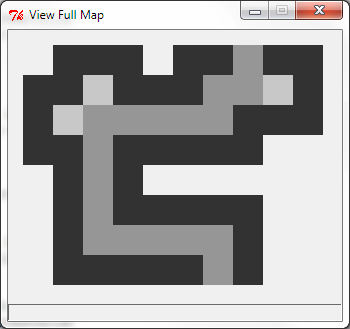
\includegraphics[width=0.35\textwidth]{entiremap.png}
\caption{Sample fully-generated map}
\end{figure}

The robot successfully explored an open area, using an obstacle avoiding algorithm. The al­gorithm consisted of a rotation function and forward function according to the structure of the surrounding environment. Firstly, it recorded obstacles and walls of the entire room. The algo­rithm divided the room into squares of identical size as the robot and fifilled it in according to the data it collected. For instance, the squares were shaded according to the image obtained from the camera which was processed onto software which displayed a 2D mapping of the area. The robot effectively utilized the infrared sensors to avoid walls and obstacles on the way. As the robot collected data on the structure of the area, updates were sent in real time to the graphical user interface and were presented in the form of a dynamic map of the area being scouted. This map contains critical information such as the location of walls, obstacles, and available paths. collecting all the required data, the program built an image representation of the floor plan of the area, indicating where walls and obstacles are. As a result of this, our robot was capable of obtaining critical information such as the location of walls, obstacles, and critical loca­tions containing very bright light, such as a fire. The map was available on the computer screen on-demand after the robot had finished exploring an area.\\

\begin{figure}[ht]
\centering
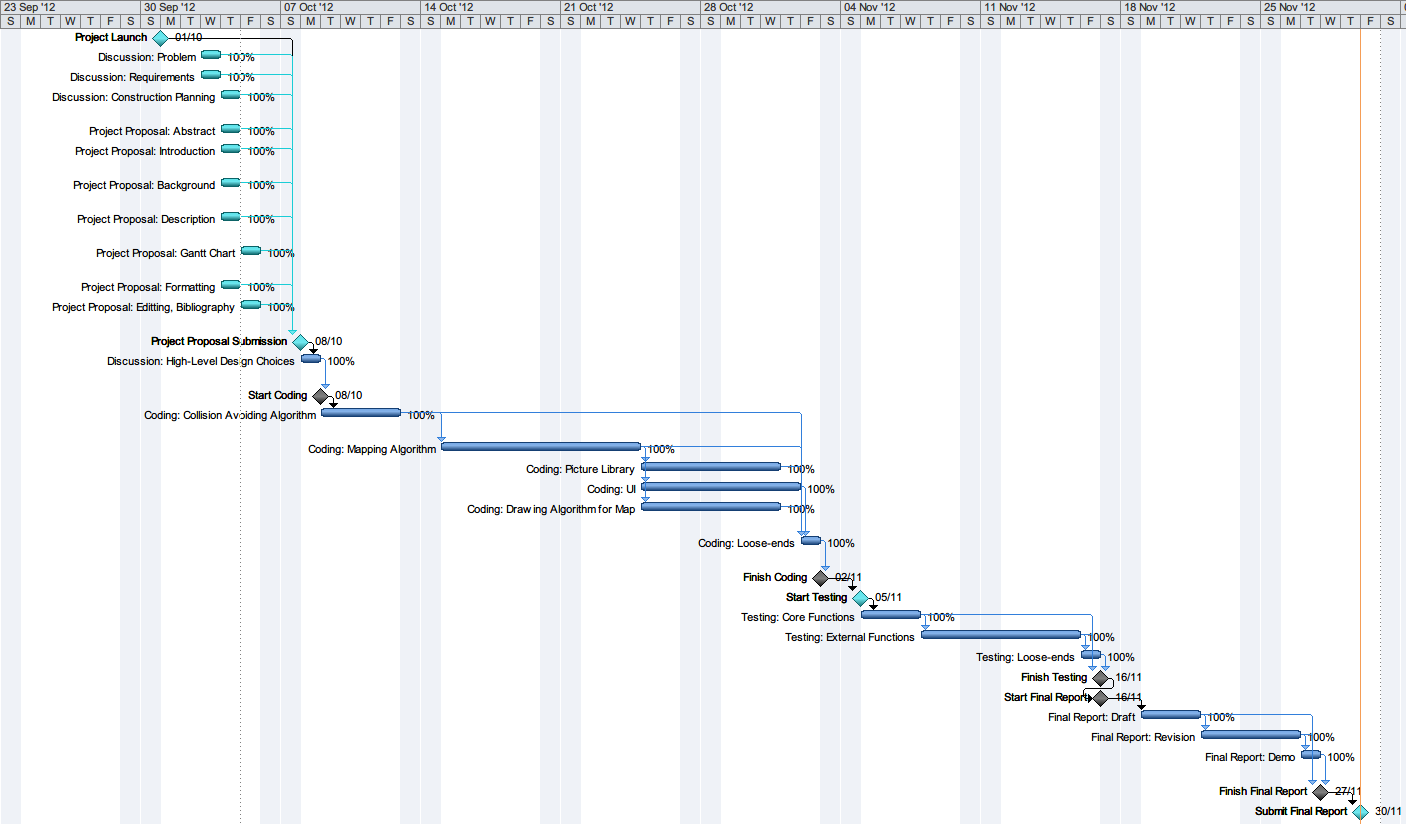
\includegraphics[width=0.8\textwidth]{gannt.png}
\caption{Gannt Chart of our project's progress}
\end{figure}

\newpage

\section*{\fontsize{16}{16}\textsf{2 Problem Description}}
\addcontentsline{toc}{section}{Problem Description}
\onehalfspacing

The history of humanity is defined by man's eternal quest for discovery. However there are times in which it would be unwise to risk human lives in the exploration of an unknown location. The advent of technology has brought forth new ways in which we are able to perform tasks with minimal risk to human life and property.\\

Currently, there are variety of tasks unsafe or impractical for humans to perform. For example, firefighters going inside a burning buildings to rescue civilians, miners travelling deep into unstable mines. Our project group has realized there are a lot of places where we cannot reach due to hazards or the constraints of the infrastructure. We decided to program our robot to go into a room and map it out so that we will know how the area is configured without actually having humams go into the room. The robot will scout through the entire room and record where obstacles are, then it'll print it out the map of the room on the user's computer. In addition, this technology can help a lot of people when there are natural disasters because humans rely on their vision, which can be innacurate, whereas the robot's IR sensor can often obtain more pertinent and/or accurate information. The practical applications of this robot are varied and multifaceted, and it would thus be a great use in preserving human health and property.\\

\newpage

\section*{\fontsize{16}{16}\textsf{3 Design Constraints and Criteria Description}}
\addcontentsline{toc}{section}{Design Constraints and Criteria Description}
\onehalfspacing

The robot must be able to avoid all the obstacles, so it should never make contact with any object. It must explore the entire area and then generate a map with high fidelity. The shape and the size of the map should match that of the area explored with all the obstacles the scribbler encountered clearly marked on the map. The robot should accomplish its task automatically, and without human control. The robot should accomplish this task with a time limit of half of a minute per square meter (30 $\frac{s}{m^2}$).

\newpage

\section*{\fontsize{16}{16}\textsf{4 Analysis and Design}}
\addcontentsline{toc}{section}{Analysis and Design}
\onehalfspacing

In the process of programming the scribbler robot, several obstacles were encountered. Programming wise, the main problem was setting the size of 2D array. Since the size of the room was an unknown, the size of array had to be enlarged as the robot scouted the unknown room. Thankfully, Python has a built-in append function which increases the size of the array dynamically\cite{kun}. Therefore, it was possible to dynamically allocate memory and reset the size of the array.\\

Working with the scribbler, our group realized that the robot was far from perfect. One critical problem was that we could not get the robot to turn exactly 90 degrees. After a few turns, we can observe that the scribbler robot is no longer aligned with its original orientation. Since we must calculate the position of the robot, as soon as the robot goes off trail by turning imprecisely, it renders our outputted data inconsistent. The first solution was to time the robot as it turns to determine how much time is required to turn exactly 90$^\circ$. This method did not seem to be effective, thus we switched to a completely different method where we used the robot’s rotary encoders within its wheels to determine how much it had turned. This method proved to be much more effective than timing the rotations. This methodology made turns much more precise, though there were still slight innacuracies.\\

\begin{table}[ht]
\centering
  \caption{Measurements of the scribbler's turning angle with the turn() series of functions included in the Myro library. Speed setting is 0.5}
  \begin{tabular}{clc}
  Time (s) & Direction & Turn Amount ($^\circ$) \\ \hline
  1.300    & Left      & 85                     \\
  1.350    & Left      & 87                     \\
  1.380    & Left      & 88                     \\
  1.399    & Left      & 89                     \\
  1.400    & Left      & 91                     \\
  1.300    & Right     & 85                     \\
  1.350    & Right     & 87                     \\
  1.380    & Right     & 88                     \\
  1.400    & Right     & 89                     \\
  1.401    & Right     & 91                     \\ \hline
  \end{tabular}
\end{table}

Finally, one of the worst problems we faced was accuracy problem with the IR sensors. Sometimes, they would detect an object from 10 cm away and sometimes they would detect that same object from 30 cm away. Because of this, the robot could not always perfectly map out the room since it would sometimes recognize an object from far away, making that object seem bigger than it was. To fix this, power going to the IR sensors was reduced, just enough to detect only objects that are in close range. However, we could not fully fix this problem: the IR sensors were accurate most of the time, but there still were a few times where they sensed objects from a far distance away. Unfortunately, this would cause even perfectly straight walls to sometimes appear as jagged lines on our map.\\

\begin{table}[ht]
\centering
  \caption{Test data of the fluke's IR Obstacle Detector. All tests made while the robot is stationary. All data taken as an average of 3 consecutive readings.}
  \begin{tabular}{ccccc}
  Distance (m) & IR Power & Sensor 1 & Sensor 2 & Sensor 3 \\ \hline
  0.05         & 125      & 255      & 482      & 225      \\
  0.10         & 125      & 0        & 0        & 0        \\
  0.10         & 130      & 755      & 1132     & 476      \\
  0.10         & 130      & 1113     & 1076     & 123      \\
  0.15         & 130      & 544      & 735      & 497      \\
  0.20         & 130      & 0        & 0        & 0        \\
  0.15         & 135      & 356      & 788      & 592      \\
  0.15         & 135      & 630      & 1142     & 576      \\
  0.20         & 135      & 312      & 773      & 332      \\
  0.25         & 135      & 0        & 0        & 0        \\ \hline
  \end{tabular}
\end{table}

On the positive side, our completed design was able to generate a map of its surroundings in real-time, which was an improvement over our original plans.\\

\begin{figure}[ht]
\centering
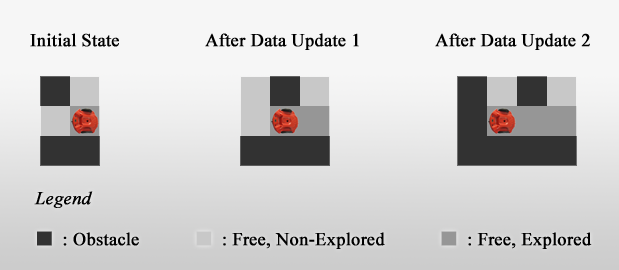
\includegraphics[width=0.9\textwidth]{realtimetracking.png}
\caption{Sample step-by-step map output}
\end{figure}

The bulk of any potential improvements to our design must be done through altered hardware. For example, if the scribbler's IR sensors could give consistent readings, much of our imprecise data could be rendered more accurate. Another possible hardware improvement would be an on-board gyroscope, to make sure that the scribbler would have the increased accuracy which is a direct product of being more stable. This would also help to solve the problems with inaccurate turning.\\

\newpage

\section*{\fontsize{16}{16}\textsf{5 Scope and Depth of Report}}
\addcontentsline{toc}{section}{Scope and Depth of Report}
\onehalfspacing

\subsection*{\fontsize{14}{14}\textsf{Scope}}
\addcontentsline{toc}{subsection}{Scope}
\onehalfspacing
Time and cost are two crucial factors which control our modern world project structures. By defining the scope of a project, we can optimize the efficiency both financially and functionally by ensuring the project creation process follows the required design scheme.\\

The area of exploration or examination was limited to 50 m$^2$ . This limitation defines and consequently measures the necessary amount of power and the duration of our robot’s tasks, which ultimately defines the time and cost associated with our robot model project. In addition, the floor map is to include only critical information such as corners, obstacles and critical locations containing very bright light, such as fire. In addition, the floor map of the area is to be displayed in black and white, to produce a simple map containing critical information such as corners, obstacles and critical locations containing very bright light, such as fifire. This allows for diversity in the types of software that can be used to successfully carry out our goal function. Moreover, it makes the mapping process much simpler as it requires minimal sensor-graphic usage, which leads to saving energy due to the reduced amount of power used. \\

The main robot model used to carry out our task in this project is referred as the Scribbler, a multifunctioning robot. Its wide range of functions, such as a camera, movement ability, IR sensors, and picture processing allows us to effectively carry out our task both financially and functionally. In addition, the scribbler robot defifines the main cost required for this project, because all other work is done through software and programming which requires minimal financial enumeration. For instance, the Python programming language is used to program the scribbler’s motion and map generating functions. There is no cost associated with the use of this language, which makes cost a negligible factor for a signifificant portion of our project, the software.\\

The previously discussed scopes provide a good approximation of the cost and time associated with our project. The duration of the map-generating task is defined and the corresponding energy or power source necessary for the job is defined. In addition, the costs of the materials required for our project are defined.\\

\subsection*{\fontsize{14}{14}\textsf{Depth}}
\addcontentsline{toc}{subsection}{Depth}
\onehalfspacing
The robot project generated diverse results ranging from the functional aspect of the project to the exploration of engineering principles and ethics in reference to the software engineering course. We were able to explore and practice many engineering principles and ethics we learned in the software engineering course. Firstly, this project provided a great team working experience through which we learned how to effectively cooperate with other fellow colleagues. Secondly, during the process of the project, fundamental engineering disciplines such as environmental awareness and decision making were practiced as well. For instance, we carefully considered not only cost and time efficiency, but also environmental efficiency by controlling amount of power used for the task. Lastly, the software developing experience was particularly significant, since it is the basic fundamental that shapes the uniqueness of software engineering.\\

The functionality of the robot was sufficiently close to our goals. We will now compare and contrast our operation objectives and results. Firstly, the robot both successfully and effectively avoided obstacles by utilizing its rotating motion and sensor functions. Secondly, the robot successfully captured the image of the obstacles and displayed in a grid system by checking the light intensity of the camera. Lastly, the robot was able to adapt to different environment with different obstacles within the open area effectively. To a great extent the project was a success, nevertheless there were minor errors and unachieved functional goals. Firstly, the sound function of beeping was removed from our robot, because it was simply energy absorbing and useless. For instance, when the robot is checking the structural design of the room (wall), it will simply beep every time it senses the wall of the room. Secondly, the image taking function was removed simply because the graphics of each obstacle are not necessary in our task and it consumes much more memory and energy when being processed. Lastly, due to the lack of efficiency of the IR sensor we were unable to avoid complex obstacles. Consequently, the project was not perfect in the functional aspect but it was nevertheless a prodigious and valuable experience.\\

\newpage

\addcontentsline{toc}{section}{References\cite{ieee}}
\begin{thebibliography}{9}

\bibitem{parallax}
  Parallax Inc. (2012, November 30). \textit{The Scribbler: A Reprogrammable Robot} [Online]. Available: http://parallax.com/

\bibitem{kun}
  Jeremy Kun. (2012, January 12). \textit{A Spoonful of Python (and Dynamic Programming)}. [Online]. Available: http://jeremykun.wordpress.com/

\bibitem{andrews}
  Gordon C. Andrews et al., \textit{Introduction to Professional Engineering in Canada}, 3rd ed., Canada: Pearson, 2009.

\bibitem{ieee}
  D. Graffox. (2009, September). \textit{IEEE Citation Reference}. [Online]. Available: http://www.ieee.org/

\end{thebibliography}

\end{document}
